\usetikzlibrary{decorations.pathmorphing}
\usetikzlibrary{decorations.markings}
\usetikzlibrary{decorations.pathmorphing}
\usetikzlibrary{arrows}
\usetikzlibrary{automata}
\usetikzlibrary{patterns}


\newlength{\hatchspread}
\newlength{\hatchthickness}
\newlength{\hatchshift}
\newcommand{\hatchcolor}{}
% declaring the keys in tikz
\tikzset{hatchspread/.code={\setlength{\hatchspread}{#1}},
         hatchthickness/.code={\setlength{\hatchthickness}{#1}},
         hatchshift/.code={\setlength{\hatchshift}{#1}},% must be >= 0
         hatchcolor/.code={\renewcommand{\hatchcolor}{#1}}}
% setting the default values
\tikzset{hatchspread=4pt,
         hatchthickness=0.8pt,
         hatchshift= 2pt,% must be >= 0
         hatchcolor=black!50}
% declaring the pattern
\pgfdeclarepatternformonly[\hatchspread,\hatchthickness,\hatchshift,\hatchcolor]% variables
   {custom north west lines}% name
   {\pgfqpoint{\dimexpr-2\hatchthickness}{\dimexpr-2\hatchthickness}}% lower left corner
   {\pgfqpoint{\dimexpr\hatchspread+2\hatchthickness}{\dimexpr\hatchspread+2\hatchthickness}}% upper right corner
   {\pgfqpoint{\dimexpr\hatchspread}{\dimexpr\hatchspread}}% tile size
   {% shape description
    \pgfsetlinewidth{\hatchthickness}
    \pgfpathmoveto{\pgfqpoint{0pt}{\dimexpr\hatchspread+\hatchshift}}
    \pgfpathlineto{\pgfqpoint{\dimexpr\hatchspread+0.15pt+\hatchshift}{-0.15pt}}
    \ifdim \hatchshift > 0pt
      \pgfpathmoveto{\pgfqpoint{0pt}{\hatchshift}}
      \pgfpathlineto{\pgfqpoint{\dimexpr0.15pt+\hatchshift}{-0.15pt}}
    \fi
    \pgfsetstrokecolor{\hatchcolor}
%    \pgfsetdash{{1pt}{1pt}}{0pt}% dashing cannot work correctly in all situation this way
    \pgfusepath{stroke}
   }

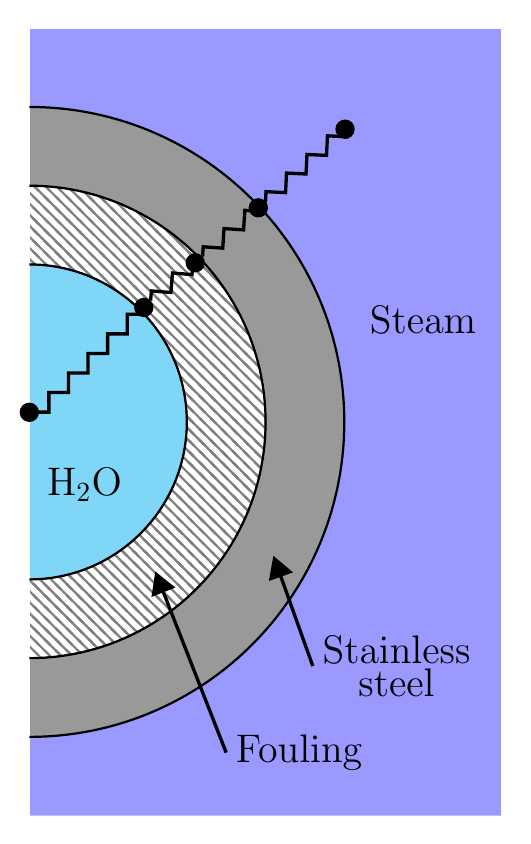
\begin{tikzpicture}[>=triangle 60]

%fill
\draw[fill=cyan!50,even odd rule] (0,-1) arc (-90:90:2);

\draw[pattern=custom north west lines, pattern color=black, even odd rule] (0,-1) arc (-90:90:2) (0,-2) arc (-90:90:3); 

\draw[fill=black!40, even odd rule] (0,-2) arc (-90:90:3) (0,-3) arc (-90:90:4); 

\draw[fill=blue!40,draw=white!0, even odd rule] (0,-3) arc (-90:90:4) rectangle (0,-4)--(0,6)--(6,6)--(6,-4); 

%contour
\draw[thick] (0,-1) arc (-90:90:2); 

\draw[ thick] (0,-2) arc (-90:90:3); 

\draw[ thick] (0,-3) arc (-90:90:4); 

%resistor symbol

\coordinate (a) at (0,1);
\coordinate (b) at (1.54,2.54) {} {};
\coordinate (c) at (2.2,3.1) {} {};
\coordinate (d) at (3,3.8) {} {};
\coordinate (e) at (4.1,4.8) {} {};

\draw[*-*,very thick, decorate,decoration=zigzag] (a)--(b);
\draw[-*,very thick, decorate,decoration=zigzag] (b)--(c);
\draw[-*,very thick, decorate,decoration=zigzag] (c)--(d);
\draw[-*,very thick, decorate,decoration=zigzag] (d)--(e);

% names

\node [anchor=center] at (0.7,0.2) {\Large H$_2$O}; 

\node [anchor=center] at (5,2.3) {\Large Steam}; 

\draw[very thick,->] (2.5,-3.2)--(1.6,-0.9);
\node [anchor=west] at (2.5,-3.2) {\Large Fouling}; 

\draw[very thick,->] (3.6,-2.1)--(3.1,-0.7);
\node [anchor=west,align=center] at (3.6,-2.1) {\Large Stainless\\ \Large steel}; 

\end{tikzpicture}